\documentclass[10pt, aspectratio=169, compress, protectframetitle, handout]{beamer}
\usepackage[utf8]{inputenc}
\usepackage[english]{babel}
\usepackage{appendixnumberbeamer}
% handout to deactivate \uncover
% usetitleprogressbar might be needed
%\usepackage{beamerprosper}
\usepackage{comment}
% Load BEFORE the theme
\usepackage[normalem]{ulem}
\usepackage[T1]{fontenc}

\usetheme[progressbar=frametitle,block=fill,numbering=fraction]{metropolis}
\setbeamertemplate{blocks}[rounded][shadow=true]
%\setbeamertemplate{note page}[plain]
%\setsansfont[
%     Extension      = .otf,
%     UprightFont    = *-Light,
%     ItalicFont     = *-LightItalic,
%     BoldFont       = *-Regular,
%     BoldItalicFont = *-RegularItalic
% ]{FiraSans}
%\setmonofont[
%     Extension   = .otf,
%     UprightFont = *-Regular,
%     BoldFont    = *-Medium
%]{FiraMono}


\newcommand{\putbg}{\usebackgroundtemplate{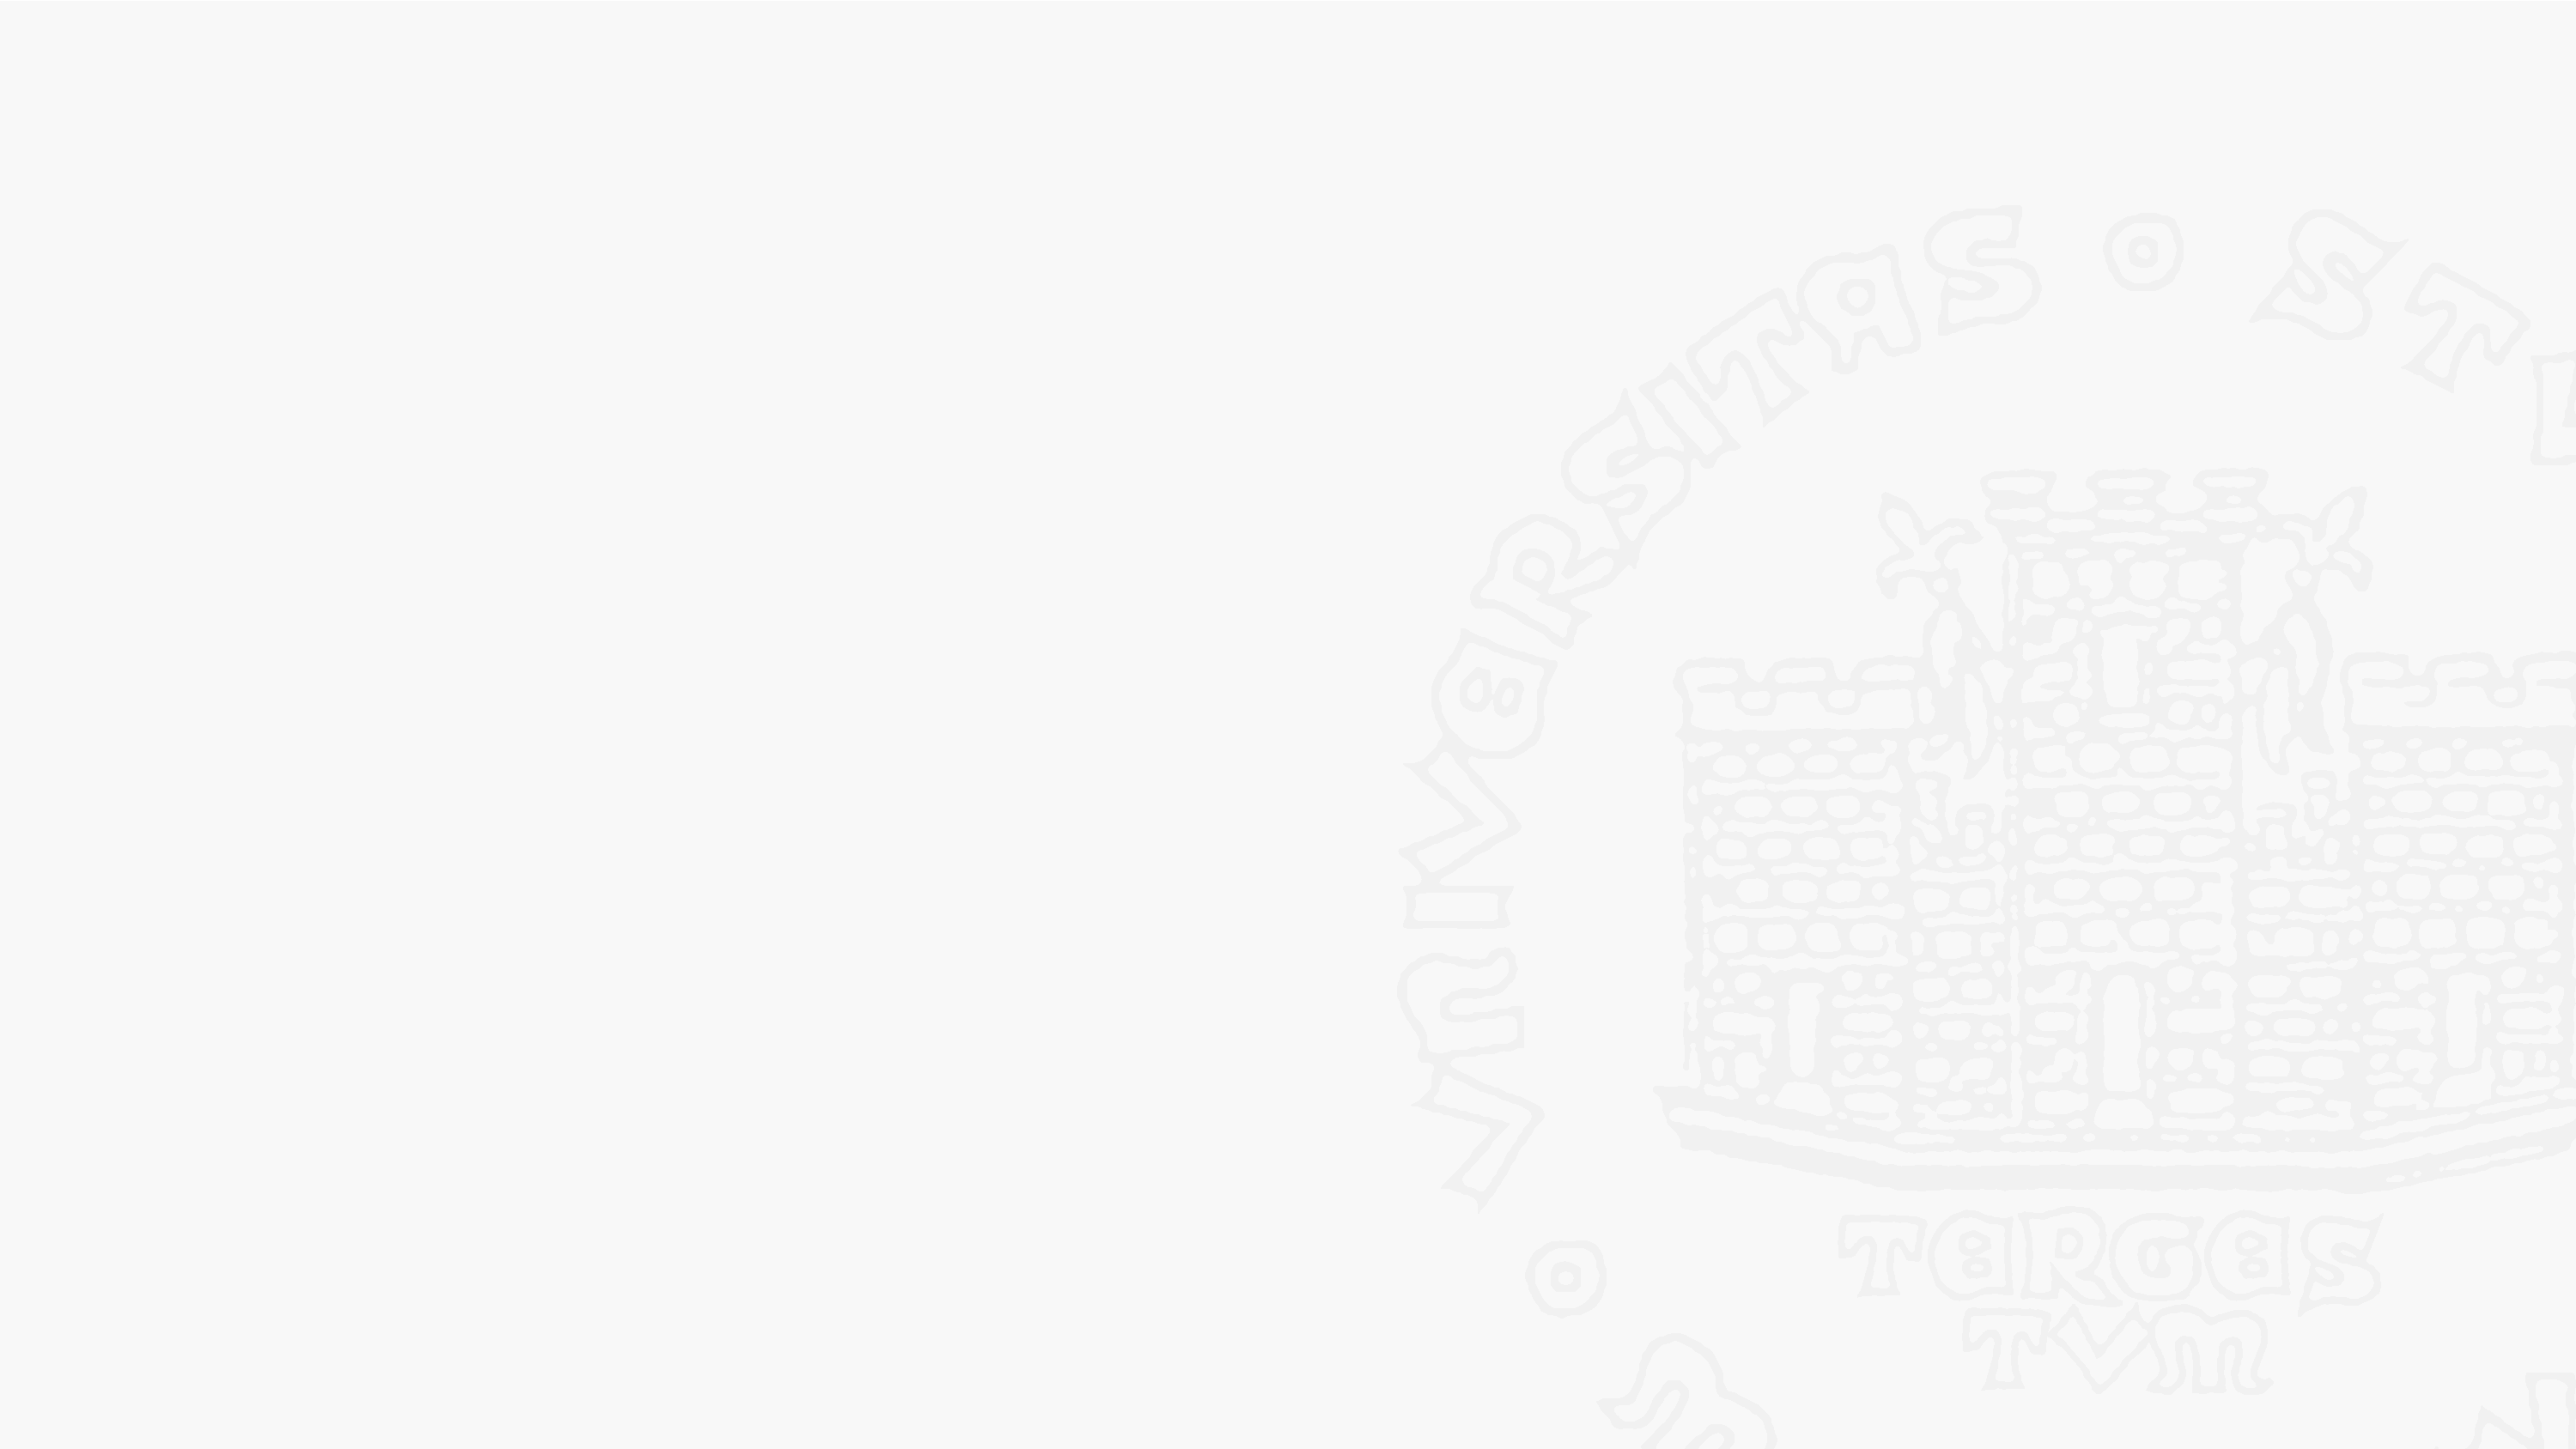
\includegraphics[width=\paperwidth,height=\paperheight]{background-vector_169}}}
\newcommand{\putbgdark}{\usebackgroundtemplate{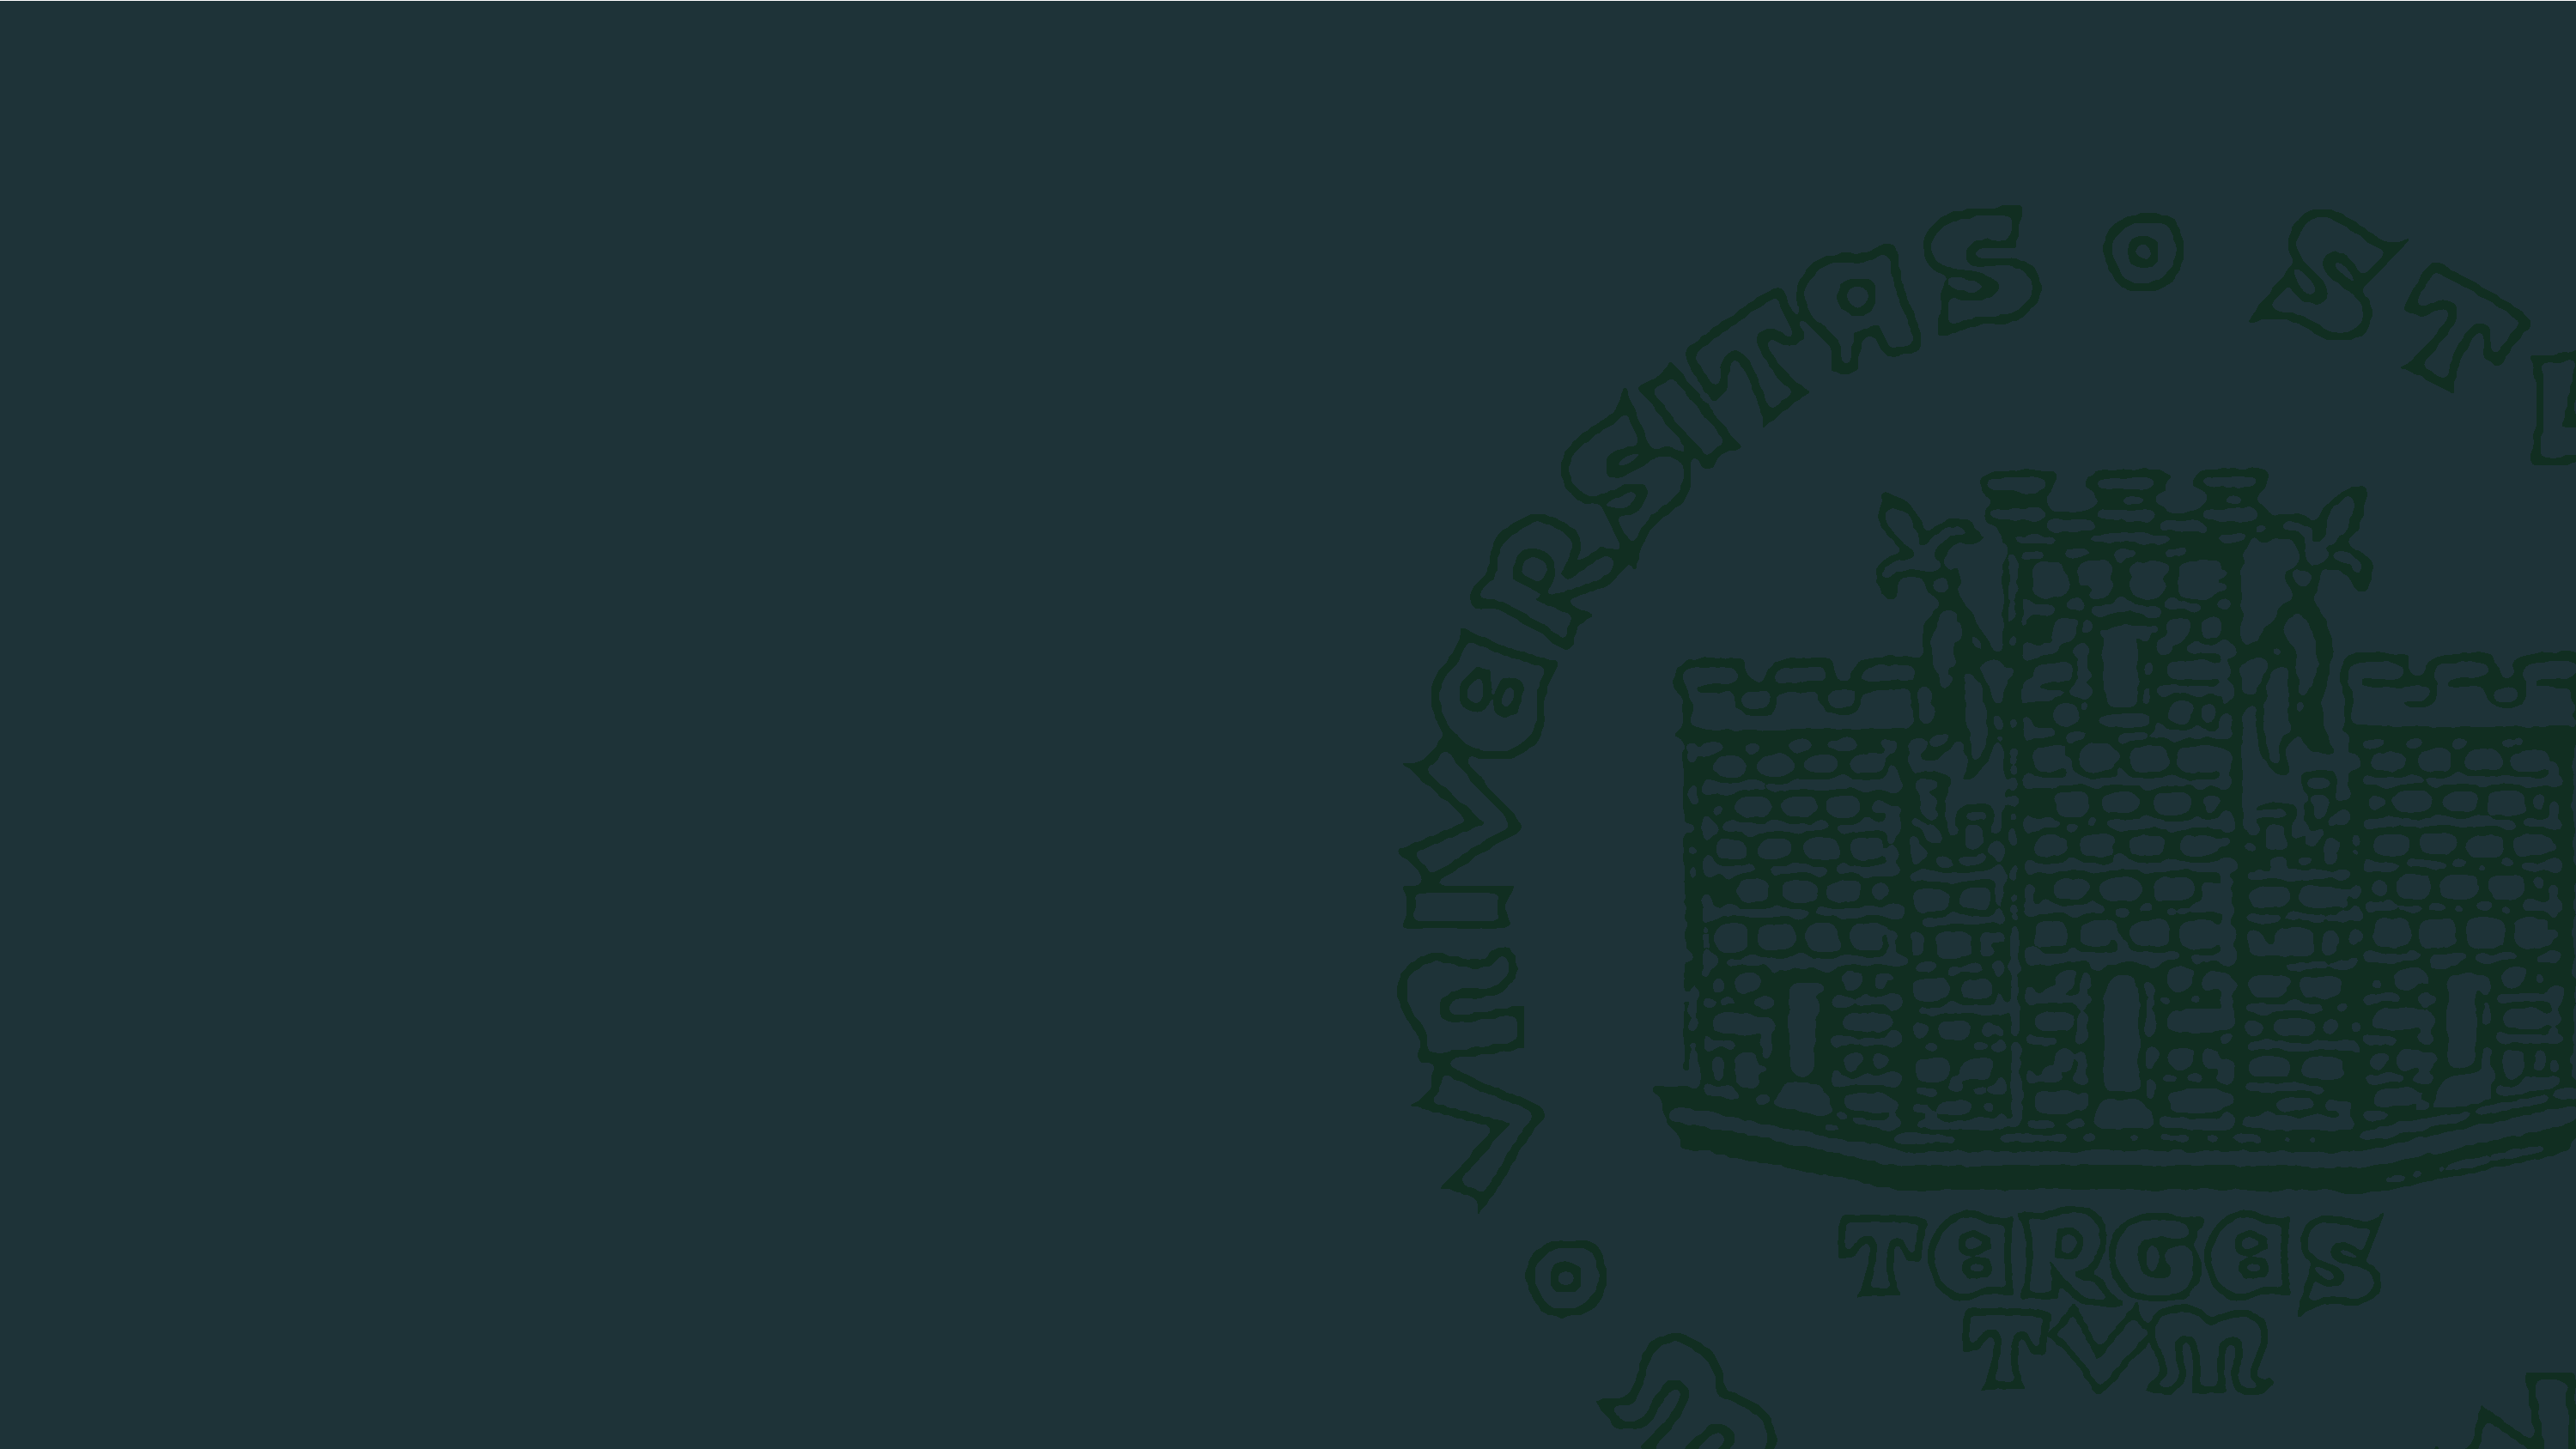
\includegraphics[width=\paperwidth,height=\paperheight]{background-vector-dark_169}}}


\usepackage[export]{adjustbox}
\usepackage[]{enumitem}
\usepackage{datetime}
\usepackage{textpos}
\usepackage{marvosym} % Smile
% Fixes bad positioning of hats
\usefonttheme{professionalfonts}%[onlymath]{serif}
\PassOptionsToPackage{hyphens}{url}\usepackage{hyperref} % to break the links
\hypersetup{
    colorlinks=true,
    linkcolor=,      % color of internal links
    urlcolor=blue,   % color of external links
    citecolor=blue,  % color of links to bibliography
}


%%% Bibliografia
\usepackage[autostyle]{csquotes}
\usepackage[backend=biber]{biblatex}
\addbibresource{biblio.bib}


%%% Metadati
\graphicspath{{figures/PNG/}{figures/PDF/}{figures/}}
\newdateformat{monthyear}{\monthname[\THEMONTH] \THEYEAR}
\title{\vspace*{1.5cm}An algorithmic reasoning approach to GNNs}
\subtitle{A project for the \emph{Deep Learning} course}
\author{Angela Carraro, Matteo Scorcia}
\date{}
\institute{\scshape DSSC + IN20 - UniTS
\vfill

\includegraphics[valign=c, height=0.7cm]{logo_dssc_alt}
\hspace*{0.5cm}
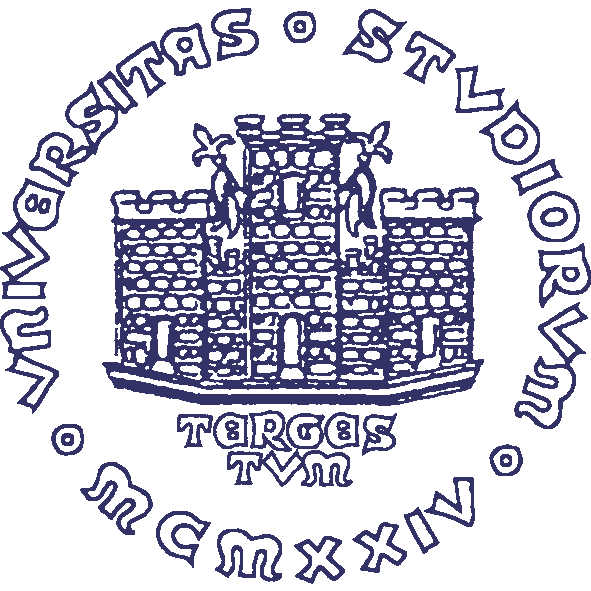
\includegraphics[valign=c, height=0.75cm]{Logo_units_blu}
}

\addtobeamertemplate{frametitle}{}{%
\begin{textblock*}{100mm}(0.90\textwidth,-0.94cm)
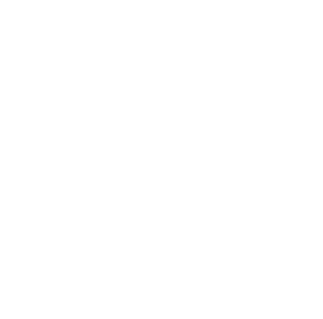
\includegraphics[valign=c, height=0.4cm]{logo_dssc_alt_white}
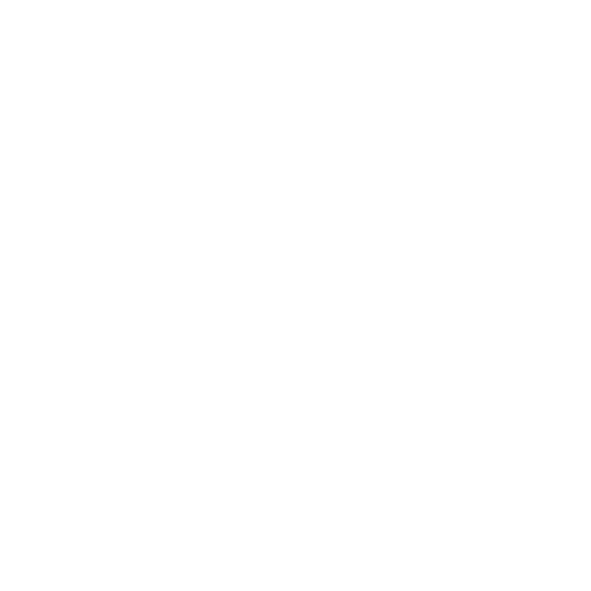
\includegraphics[valign=c, height=0.45cm]{Logo_units_white}
\end{textblock*}}

\begin{document}

{\putbg\maketitle}


%\begin{frame}{Contents}
%	\tableofcontents
%\end{frame}


\begin{frame}{Aim of the project}

    \alert{Graph Neural Networks} can have a lot of meanings, there isn't just one architecture that can be recognized as “GNN”. We will try to understand the general, abstract structure of a GNN that is presented in the book \cite{HamiltonGRLBook} (which also includes \cite{battaglia2018relational}) and to shed light about the relational inductive bias and combinatorial generalization of a GNN.
    
    Our motivation is to better understand the extent to which graph neural networks are capable of \textbf{precise and logical reasoning}.
    
\end{frame}


{\putbg
\section{Graph Theory}
}


\begin{frame}{Inroduction}
    
    Graphs are a widespread data structure and a universal language for describing and modelling complex systems. In the most general view, a graph is simply a collection of objects (i.e., nodes), along with a set of interactions (i.e., edges) between pairs of these objects. 

    \begin{columns}[onlytextwidth]
        \begin{column}{.5\textwidth-.25cm}
            Graphs are an important building block since they can naturally encode an \alert{entity-relationship structure}, as well as an \alert{invariance to permutations} (of both nodes and edges) and awareness of \alert{input sparsity}.
        \end{column}
        \begin{column}{.5\textwidth-.25cm}
            \begin{figure}
                \centering
                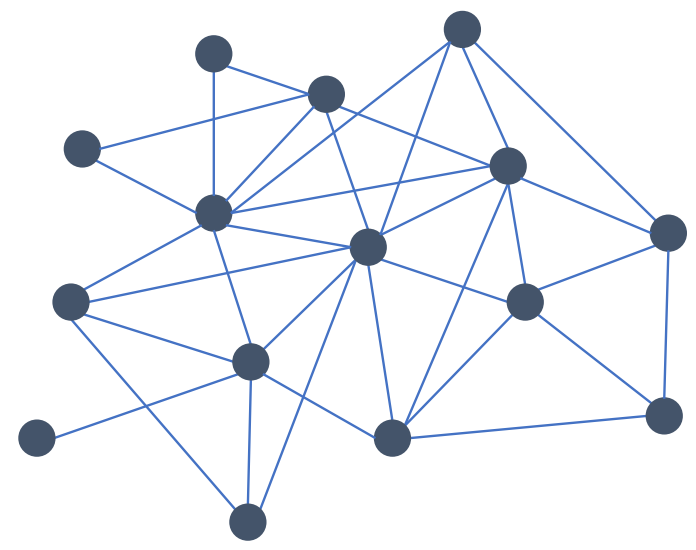
\includegraphics[width=3.8cm]{figures/Graph}
                \caption{A graph.}
            \end{figure}
        \end{column}
    \end{columns}
    
\end{frame}


\begin{frame}{Basics}
    
    \begin{block}{Definition}
        A \alert{graph} is a tuple $G = (V, E)$ where $V$ is the set of nodes and $E$ is the set of edges between these nodes. We denote an edge going from node $u \in V$ to node $v \in V$ as $(u, v) \in E$, so $E \subseteq V \times V$. The graph is \textbf{undirected} if $(u, v) \in E \Longleftrightarrow  (v, u) \in E$, otherwise it is \textbf{directed}.
    \end{block}
    
    Given a node $u$, $\mathcal N(u)$ is $u$'s graph neighborhood.
    
    A convenient way to represent graphs is through an \alert{adjacency matrix} $A \in \mathbb R^{|V| \times |V|}$, with $A[u, v] = 1$ if $(u, v) \in E$ and $A[u, v] = 0$ otherwise. If the graph is undirected the matrix in \emph{symmetric}. If the graph has weighted edges we have that $A[u,v] \in \mathbb R$.
    
    We also have \alert{attribute} or \alert{feature} information associated with a graph. Most often these are \emph{node-level attributes} that we represent using a real-valued matrix $\mathbf X \in \mathbb R^{d \times |V|}$, where we assume that the ordering of the nodes is consistent with the ordering in the adjacency matrix. In some cases we even associate real-valued \emph{features with entire graphs}.
    
\end{frame}


\begin{frame}{Machine learning on graphs}
%GNN real-world applications}

    Machine learning tasks on graph data fall in one of these four categories:
    %GNNs are used for one of three tasks:
    \begin{itemize}[topsep=4pt,itemsep=8pt]
        \item[{$\bullet$}] {\makebox[3.8cm][l]{\alert{\emph{node classification}}:} predict the label $y_u$ associated with all the nodes $u \in V$}\\
        \quad $\longrightarrow$ \; E.g., predicting whether a user is a bot in a social network
        
        \item[{$\bullet$}] {\makebox[3.8cm][l]{\alert{\emph{edge prediction}}:}
        infer the edges between nodes in a graph}\\ 
        %predict if there exists an edge between two nodes}\\
        \quad $\longrightarrow$ \; E.g., content recommendation in online platforms, predicting drug side-effects, or inferring new facts in a relational databases
        
        \item[{$\bullet$}] {\makebox[3.8cm][l]{\alert{\emph{community detection}}:} infer latent community structures given only the input graph}\\
        \quad $\longrightarrow$ \; E.g.,  uncovering functional modules in genetic interaction networks, uncovering fraudulent groups of users in financial transaction networks
        
        \item[{$\bullet$}] {\makebox[3.8cm][l]{\alert{\emph{graph class./regr./clust.}}:} given a dataset of \emph{multiple different graphs}, make independent predictions specific to each graph}\\
        \quad $\longrightarrow$ \; E.g., property prediction based on molecular graph structures 
    \end{itemize}

\end{frame}


\begin{frame}{Blurring the boundaries of ML categories}

    At first glance, node classification appears to be a straightforward variation of standard supervised classification, but there are in fact important differences. The most important difference is that the nodes in a graph are not independent and identically distributed (i.i.d.). Usually, when we build supervised machine learning models we assume that each datapoint is statistically independent from all the other datapoints; otherwise, we might need to model the dependencies between all our input points. We also assume that the datapoints are identically distributed; otherwise, we have no way of guaranteeing that our model will generalize to new datapoints. Node classification completely breaks this i.i.d. assumption. Rather than modeling a set of i.i.d. datapoints, we are instead modeling an interconnected set of nodes.
    
    Of all the machine learning tasks on graphs, graph regression and classification are perhaps the most straightforward analogues of standard supervised learning. Each graph is an i.i.d. datapoint associated with a label, and the goal is to use a labeled set of training points to learn a mapping from datapoints (i.e., graphs) to labels.
    
\end{frame}


\begin{frame}{Node-level statistics and features}

    \begin{block}{Node degree}
        The \alert{degree} of a node $u \in V$ simply counts the number of edges incident to the node, so how many neighbors the node has:
        \begin{equation}
            d_u = \sum_{v \in V} A[u, v].
            \label{eq:degree}
        \end{equation}
    \end{block}
    
    To obtain a more powerful measure of \emph{importance}, we can consider various measures of what is known as \alert{node centrality}.
    
    \begin{block}{Eigenvector centrality}
        We define a node's \alert{eigenvector centrality} $e_u$ via a recurrence relation in which the node's centrality is proportional via a constant $\lambda$ to the average centrality of its neighbors:
        \begin{equation}
            e_u = \frac1\lambda \sum_{v \in V} A[u, v] e_v \; \forall u \in V \quad \Longleftrightarrow \quad \lambda \mathbf e = A \mathbf e. \; \text{ with }\mathbf u \text{ vector of node centralities}.
            \label{eq:eigencentr}
        \end{equation}
    \end{block}
    
\end{frame}


\begin{frame}{Graph-level features and graph kernels}

    \begin{block}{Bag of nodes}
        The simplest approach to defining a graph-level feature is to just aggregate node-level statistics. For example, one can compute histograms or other summary statistics based on the degrees, centralities, and clustering coefficients of the nodes in the graph. This aggregated information can then be used as a graph-level representation. The downside to this approach is that it is entirely based upon local node-level information and can miss important global properties in the graph.
    \end{block}
    
    \begin{block}{The Weisfeiler-Lehman kernel}
        One way to improve the basic bag of nodes approach is using a strategy of \emph{iterative neighborhood aggregation}. The idea with these approaches is to extract node-level features that contain more information than just their local ego graph, and then to aggregate these richer features into a graph-level representation.

        Perhaps the most important and well-known of these strategies is the WeisfeilerLehman (WL) algorithm and kernel.
    \end{block}
    
\end{frame}


\begin{frame}{Neighborhood Overlap Detection}

    The various statistical measures of neighborhood overlap between pairs of nodes quantify the extent to which a pair of nodes are related. For example, the simplest \alert{neighborhood overlap measure} just counts the number of neighbors that two nodes share:
    \begin{equation}
        \mathbf S[u, v] = |\mathcal N(u) \cap \mathcal N(v)|,
    \end{equation}
    where we use $\mathbf S[u, v]$ to denote the value quantifying the relationship between nodes $u$ and $v$ and let $\mathbf S \in \mathbb R^{|V| \times |V|}$ denote the \alert{similarity matrix} summarizing all the pairwise node statistics.
    
    Even though there is no ``machine learning'' involved in any of the statistical measures discussed in this section, they are still very useful and powerful baselines for relation prediction. Given a neighborhood overlap statistic $\mathbf S[u, v]$, a common strategy is to assume that the likelihood of an edge $(u, v)$ is simply proportional to $\mathbf S[u, v]$:
    \begin{equation}
        \mathbf P (A[u, v] = 1) \propto \mathbf S[u, v].
    \end{equation}
    Thus, in order to approach the relation prediction task using a neighborhood overlap measure, one simply needs to set a threshold to determine when to predict the existence of an edge. Note that in the relation prediction setting we generally assume that we only know a subset of the true edges $E_\text{train} \subset E$. Our hope is that \alert{node-node similarity measures} computed on the training edges will lead to accurate predictions about the existence of test (i.e., unseen) edges.
    
\end{frame}


\begin{frame}{?????????}

    In the previous sections, we saw a number of traditional approaches to learning over graphs. However, the approaches discussed --- and especially the node and graph-level statistics --- are limited due to the fact that they require careful, hand-engineered statistics and measures. We will introduce an alternative approach to learning over graphs: \alert{graph representation learning}. Instead of extracting hand-engineered features, we will seek to \emph{learn} representations that encode structural information about the graph.
    
\end{frame}


{\putbg
\section{Neighborhood Reconstruction Methods}
}


\begin{frame}{Frame Title}

    \begin{columns}[onlytextwidth]
        \begin{column}{.4\textwidth-.25cm}
        We will now see methods for learning \alert{node embeddings}. The goal of these methods is to encode nodes as low-dimensional vectors that summarize their graph position and the structure of their local graph neighborhood. In other words, we want to project nodes into a latent space, where geometric relations in this latent space correspond to relationships (e.g., edges) in the original graph or network.
        \end{column}
        \begin{column}{.6\textwidth-.25cm}
        \begin{figure}[ht]
            \centering
            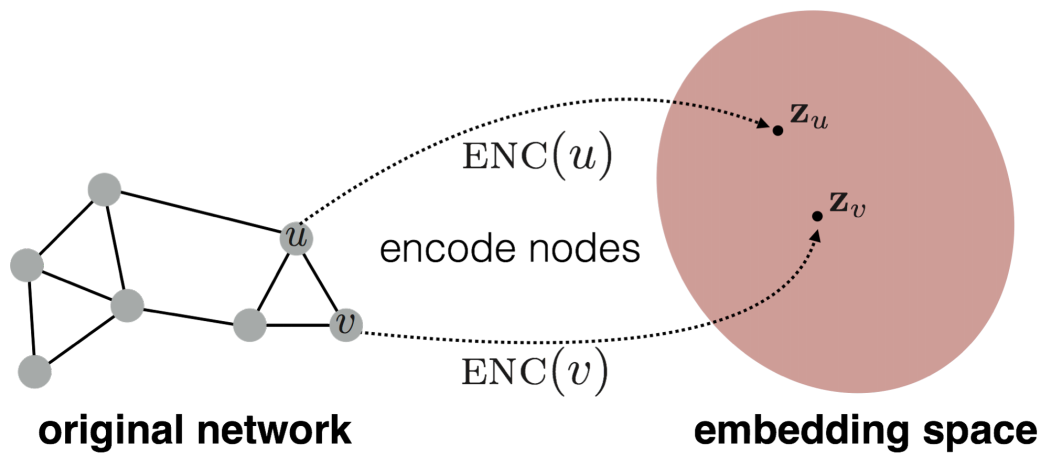
\includegraphics[width=8cm]{figures/Node_embedding.png}
            \caption{Illustration of the node embedding problem. Our goal is to learn an encoder (enc), which maps nodes to a low-dimensional embedding space. These embeddings are optimized so that distances in the embedding space reflect the relative positions of the nodes in the original graph.}
            \label{fig:nodeembedding}
        \end{figure}
        \end{column}
    \end{columns}
    
\end{frame}


\begin{frame}{An Encoder-Decoder Perspective}

    We organize our discussion of node embeddings based upon the framework of \alert{encoding and decoding graphs}. In the encoder-decoder framework, we view the graph representation learning problem as involving two key operations. First, an \alert{encoder} model maps each node $u$ in the graph into a low-dimensional vector or embedding $\mathbf z_u$. Next, a \alert{decoder} model takes the low-dimensional node embeddings $\mathbf z_u$ and uses them to reconstruct information about each node $u$'s neighborhood in the original graph.

    \begin{figure}[ht]
        \centering
        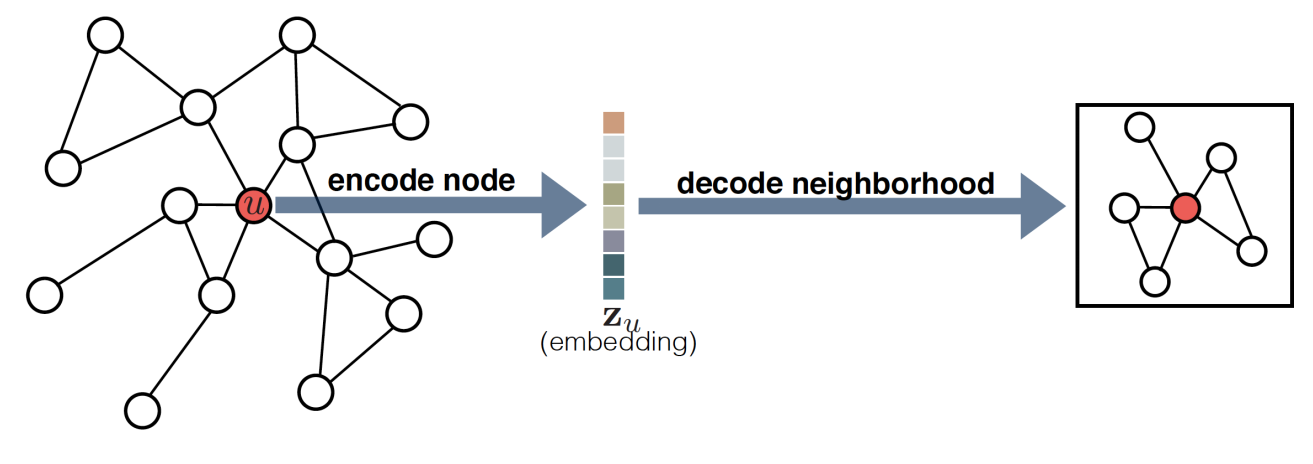
\includegraphics[width=10cm]{figures/Encoder_decoder.png}
        \label{fig:enc-dec}
    \end{figure}
    
\end{frame}


\begin{frame}{The Encoder}

    Formally, the \alert{encoder} is a function that maps nodes $v \in V$ to vector embeddings $\mathbf z_v \in \mathbb R^d$ (where $\mathbf z_v$ corresponds to the embedding for node $v \in V$). In the simplest case, the encoder has the following signature:
    \begin{equation}
        \textsc{enc}: V \rightarrow \mathbb R^d,
    \end{equation}
    meaning that the encoder takes node IDs as input to generate the node embeddings. In most work on node embeddings, the encoder relies on what we call the \alert{shallow embedding} approach, where this encoder function is simply an embedding lookup based on the node ID. In other words, we have that
    \begin{equation}
        \textsc{enc}(v) = \mathbf Z[v],
        \label{eq:shallowemb}
    \end{equation}
    where $\mathbf Z \in \mathbb R^{|V| \times d}$ is a matrix containing the embedding vectors for all nodes and $\mathbf Z[v]$ denotes the row of $\mathbf Z$ corresponding to node $v$.
    
\end{frame}


\begin{frame}{The Decoder}

    The role of the \alert{decoder} is to reconstruct certain graph statistics from the node embeddings that are generated by the encoder. For example, given a node embedding $\mathbf z_u$ of a node $u$, the decoder might attempt to predict $u$'s set of neighbors $\mathcal N(u)$ or its row $A[u]$ in the graph adjacency matrix.
    
    While many decoders are possible, the standard practice is to define pairwise decoders, which have the following signature:
    \begin{equation}
        \textsc{dec}: \mathbb R^d \times \mathbb R^d \rightarrow \mathbb R^+.
    \end{equation}
    Pairwise decoders can be interpreted as predicting the relationship or similarity between pairs of nodes. For instance, a simple pairwise decoder could predict whether two nodes are neighbors in the graph.
    
    Applying the pairwise decoder to a pair of embeddings $(\mathbf z_u, \mathbf z_v)$ results in the \emph{reconstruction} of the relationship between nodes $u$ and $v$. The goal is optimize the encoder and decoder to minimize the reconstruction loss so that
    \begin{equation}
        \textsc{dec}(\textsc{enc}(u), \textsc{enc}(v)) = \textsc{dec}(\mathbf z_u, \mathbf z_v) \approx \mathbf S[u, v].
        \label{eq:reconstrloss}
    \end{equation}
    Here, we assume that $\mathbf S[u, v]$ is a graph-based similarity measure between nodes. For example, the simple reconstruction objective of predicting whether two nodes are neighbors would correspond to $\mathbf S[u, v] := A[u, v]$. However, one can define $\mathbf S[u, v]$ in more general ways as well, for example, by leveraging any of the pairwise neighborhood overlap statistics discussed earlier.
        
\end{frame}


\begin{frame}{Optimizing an Encoder-Decoder Model}

    To achieve the reconstruction objective (\autoref{eq:reconstrloss}), the standard practice is to minimize an empirical reconstruction loss $\mathcal L$ over a set of training node pairs $\mathcal D$:
    \begin{equation}
        \mathcal L = \sum_{(u,v) \in \mathcal D} \ell (\textsc{dec}(\mathbf z_u, \mathbf z_v), \mathbf S[u, v]),
        \label{eq:loss}
    \end{equation}
    where $\ell: \mathbb R \times \mathbb R \rightarrow \mathbb R$ is a loss function measuring the discrepancy between the decoded (i.e., estimated) similarity values $\textsc{dec}(\mathbf z_u, \mathbf z_v)$ and the true values $\mathbf S[u, v]$. Depending on the definition of the decoder ($\textsc{dec}$) and similarity function ($\mathbf S$), the loss function $\ell$ might be a mean-squared error or even a classification loss, such as cross entropy. Thus, the overall objective is to train the encoder and the decoder so that pairwise node relationships can be effectively reconstructed on the training set $\mathcal D$. Most approaches minimize the loss in \autoref{eq:loss} using stochastic gradient descent, but there are certain instances when more specialized optimization methods (e.g., based on matrix factorization) can be used.
    
\end{frame}


\begin{frame}{Limitations of Shallow Embeddings}

    This focus of this chapter has been on shallow embedding methods. In these approaches, the encoder model that maps nodes to embeddings is simply an embedding lookup (\autoref{eq:shallowemb}), which trains a unique embedding for each node in the graph. However, it is also important to note that shallow embedding approaches suffer from some important drawbacks:
    \begin{itemize}
        \item[\alert{$\bullet$}] The first issue is that they do not share any parameters between nodes in the encoder, since the encoder directly optimizes a unique embedding vector for each node. This lack of parameter sharing is both statistically and computationally inefficient.
        \item[\alert{$\bullet$}] A second key issue is that they do not leverage node features in the encoder.
        \item[\alert{$\bullet$}] Lastly --- and perhaps most importantly --- they are inherently \emph{transductive}. These methods can only generate embeddings for nodes that were present during the training phase. Generating embeddings for new nodes --- which are observed after the training phase --- is not possible unless additional optimizations are performed to learn the embeddings for these nodes. This restriction prevents shallow embedding methods from being used on \emph{inductive} applications, which involve generalizing to unseen nodes after training.
    \end{itemize}

    To alleviate these limitations, shallow encoders can be replaced with more sophisticated encoders that depend more generally on the structure and attributes of the graph. We will discuss the most popular paradigm to define such encoders, i.e.., graph neural networks (GNNs).

\end{frame}


{\putbg
\section{The Graph Neural Network Model}
\label{sec:GNNmodel}
}


\begin{frame}{A stupid GNN}

    To define a \alert{deep neural network over graphs} one could simply use the adjacency matrix as input to a deep neural network. For example, to generate an embedding of an entire graph we could simply flatten the adjacency matrix and feed the result to a multi-layer perceptron (MLP):
    \begin{equation}
        \mathbf z_G = \text{MLP}(\mathbf A[1] \oplus \mathbf A[2] \oplus \ldots \oplus \mathbf A[|\mathcal V|]);
    \end{equation}
    where $\mathbf A[i] \in \mathbf R^{|\mathcal V|}$ denotes a row of the adjacency matrix and we use $\oplus$ to denote vector concatenation.
    
    The issue with this approach is that it \textit{depends on the arbitrary ordering of nodes that we used in the adjacency matrix}. In other words, such a model is \alert{not permutation invariant}.
    
    Any function $f$ that takes an adjacency matrix $\mathbf A$ as input should ideally satisfy one of the two following properties, given a permutation matrix $\mathbf P$:
    \begin{align}
        f(\mathbf{PAP}^T) = f(\mathbf A) \qquad &\text{(Permutation Invariance)} \\
        f(\mathbf{PAP}^T) = \mathbf P f(\mathbf A) \qquad &\text{(Permutation Equivariance)},
    \end{align}
    
\end{frame}


\begin{frame}{Neural Message Passing}

    How we can take an input graph $G = (V, E)$, along with a set of node features $\mathbf X \in \mathbb R^{d \times |V|}$, and use this information to generate node embeddings $\mathbf z_u, \forall u \in V$?
    
    During each message-passing iteration $k$ in a GNN, a \alert{hidden embedding} $\mathbf h^{(k)}_u$ corresponding to each node $u \in \mathcal V$ is updated according to information aggregated from $u$'s graph neighborhood $\mathcal N(u)$. This message-passing update can be expressed as follows:
    \begin{align}
        \mathbf h^{(k+1)}_u &= \textsc{update}^{(k)} \left( \mathbf h^{(k)}_u; \textsc{aggregate}^{(k)}(\{\mathbf h^{(k)}_v, \forall v \in \mathcal N(u)\}) \right) 
        \label{eq:mess-pass} \\
        &= \textsc{update}^{(k)} \left( \mathbf h^{(k)}_u, \mathbf m^{(k)}_{\mathcal N(u)} \right),
        \label{eq:mess-pass2}
    \end{align}
    where $\textsc{update}$ and $\textsc{aggregate}$ are arbitrary differentiable functions (i.e., neural networks) and $\mathbf m_{\mathcal N(u)} = \textsc{aggregate}(\{\mathbf h_v, \forall v \in \mathcal N(u)\})$ is the ``message'' that is aggregated from $u$'s graph neighborhood $\mathcal N(u)$ (\alert{neighborhood aggregation operation}). The different iterations of message passing are also sometimes known as the different ``layers'' of the GNN.

\end{frame}


\begin{frame}{Message Passing in Practice}

    The initial embeddings at k = 0 are set to the input features for all the nodes, i.e., $\mathbf h^{(0)}_u = \mathbf x_u, \forall u \in \mathcal V$. After running $K$ iterations of the GNN message passing, we can use the output of the final layer to define the \alert{embeddings} for each node, i.e.,
    \begin{equation}
        \mathbf z_u = \mathbf h^{(K)}_u, \forall u \in \mathcal V.
    \end{equation}
    Note that since the $\textsc{aggregate}$ function takes a set as input, GNNs defined in this way are permutation equivariant by design.
    
    \alert{Basic intuition} $\longrightarrow$ at each iteration, every node aggregates information from its local neighborhood, and as these iterations progress each node embedding contains more and more information from further reaches of the graph.
    
    \begin{itemize}
        \item[\alert{$\bullet$}] \emph{structural information} about the graph $\longrightarrow$ after $k$ iterations, $\mathbf h^{(k)}_u$ might encode information about the degrees of all the nodes in $u$'s $k$-hop neighborhood.
    
        \item[\alert{$\bullet$}] \emph{feature-based information} about the graph $\longrightarrow$ after $k$ iterations, $\mathbf h^{(k)}_u$ also encodes information about all the features in its $k$-hop neighborhood $\rightarrow$ analogous to convolutional kernels in CNNs!
    \end{itemize}
    
\end{frame}


\begin{frame}{The Basic GNN}

    The basic GNN message passing is defined as
    \begin{equation}
        \mathbf h^{(k)}_u = \sigma \left( \mathbf W^{(k)}_\text{self} \mathbf h_u^{(k-1)} + \mathbf W_\text{neigh}^{(k)} \sum_{v \in \mathcal N(u)} \mathbf h^{(k-1)}_v + \mathbf b^{(k)} \right),
    \end{equation}
    where $\mathbf W^{(k)}_\text{self}, \mathbf W_\text{neigh}^{(k)} \in \mathbb R^{d^{(k)} \times d^{(k-1)}}$ are trainable parameter matrices and $\sigma$ denotes an elementwise non-linearity (e.g., a tanh or ReLU). The bias term $b^{(k)} \in \mathbb R^{d^{(k)}}$ is often omitted for notational simplicity, but including it can be important to achieve strong performance.
    
    We can equivalently define the basic GNN through the \textsc{update} and \textsc{aggregate} functions:
    \begin{align}
        &\mathbf m_{\mathcal N(u)} = \sum_{v \in \mathcal N(u)} \mathbf h_v, 
        \label{eq:basicgnn} \\
        &\textsc{update}(\mathbf h_u, \mathbf m_{\mathcal N(u)}) = \sigma \left( \mathbf W_\text{self} \mathbf h_u + \mathbf W_\text{neigh} \mathbf m_{\mathcal N(u)} \right),
    \end{align}
    
    Any GNNs can also be succinctly defined using graph-level equations. In the case of a basic GNN, we can write the graph-level definition of the model as follows:
    \begin{equation}
        \mathbf H^{(k)} = \sigma \left( A \mathbf H^{(k-1)} \mathbf W_\text{neigh}^{(k)} + \mathbf H^{(k-1)} \mathbf W_\text{self}^{(k)} \right),
    \end{equation}
    where $\mathbf H^{(k)} \in \mathbb R^{|V| \times d}$ denotes the matrix of node representations at layer $k$ in the GNN (with each node corresponding to a row in the matrix), $A$ is the graph adjacency matrix, and we have omitted the bias term for notational simplicity.
    
\end{frame}


\begin{frame}{Message Passing with Self-loops}

    As a simplification of the neural message passing approach, it is common to add self-loops to the input graph and omit the explicit update step. In this approach we define the message passing simply as
    \begin{equation}
        \mathbf h^{(k)}_u = \textsc{aggregate}(\{\mathbf h_v^{(k-1)}, \; \forall v \in \mathcal N(u) \cup \{u\}\}),
    \end{equation}
    where now the aggregation is taken over the set $\mathcal N(u) \cup \{u\}$, i.e., the node’s neighbors as well as the node itself. The benefit of this approach is that we no longer need to define an explicit update function, as the update is implicitly defined through the aggregation method.
    
    In the case of the basic GNN, adding self-loops is equivalent to  sharing parameters between the $\mathbf W_\text{self}$ and $\mathbf W_\text{neigh}$ matrices, which gives the following graph-level update:
    \begin{equation}
        \mathbf H^{(k)} = \sigma \left( (A + I) \mathbf H^{(k-1)} \mathbf W^{(k)} \right) .
    \end{equation}
    In the following chapters we will refer to this as the \alert{self-loop approach}.

\end{frame}


\begin{frame}{Graph convolutional networks (GCNs)}

    The most basic neighborhood aggregation operation (\autoref{eq:basicgnn}) simply takes the sum of the neighbor embeddings. One issue with this approach is that it can be unstable and highly sensitive to node degrees. One solution to this problem is to simply \emph{normalize the aggregation operation} based upon the degrees of the nodes involved:
    \begin{equation}
        \mathbf m_{\mathcal N(u)} = \frac{\sum_{v \in \mathcal N(u)} \mathbf h_v}{|\mathcal N(u)|}.
    \end{equation}
    
    Another normalization factor is the \alert{symmetric normalization}:
    \begin{equation}
        \mathbf m_{\mathcal N(u)} = \sum_{v \in \mathcal N(u)} \frac{\mathbf h_v}{\sqrt{|\mathcal N(u)| |\mathcal N(v)|}}.
    \end{equation}
    
    The popular \alert{graph convolutional network (GCN)} employs the \emph{symmetric-normalized aggregation} as well as the \emph{self-loop approach}, using as message passing function
    \begin{equation}
        h^{(k)}_u = \sigma \left( \mathbf W^{(k)} \sum_{v \in \mathcal N(u) \cup \{u\}} \frac{\mathbf h_v}{\sqrt{|\mathcal N(u)| |\mathcal N(v)|}} \right).
    \end{equation}

\end{frame}


\begin{frame}{Improving the Aggregation Layer}

    An aggregation function with the following form is a \alert{universal set function approximator}:
    \begin{equation}
        \mathbf m_{\mathcal N(u)} = \textbf{MLP}_\theta \left( \sum_{v \in \mathcal N(u)} \textbf{MLP}_\phi (\mathbf h_v) \right).
        \label{eq:univsetapproxf}
    \end{equation}
    So any permutation-invariant function that maps a set of embeddings to a single embedding can be approximated to an arbitrary accuracy by a model following (\autoref{eq:univsetapproxf}).\\
    $\longrightarrow$ \alert{set pooling} leads small increases in performance but increased risk of overfitting
    
    Another strategy is to apply \alert{attention}: assign an attention weight or importance to each neighbor, which is used to weigh this neighbor’s influence during the aggregation step. The first GNN model to apply this style of attention was the \alert{Graph Attention Network (GAT)}:
    \begin{equation}
        \mathbf m_{\mathcal N(u)} = \sum_{v \in \mathcal N(u)} \alpha_{u,v} \mathbf h_v,
    \end{equation}
    where $\alpha_{u,v}$ denotes the attention on neighbor $v \in \mathcal N(u)$ (\emph{neighborhood attention}) when we are aggregating information at node $u$.
    
\end{frame}


\begin{frame}{Visualize a single GAT step}

    \begin{columns}[onlytextwidth]
        \begin{column}{.5\textwidth}
            \begin{figure}
                \centering
                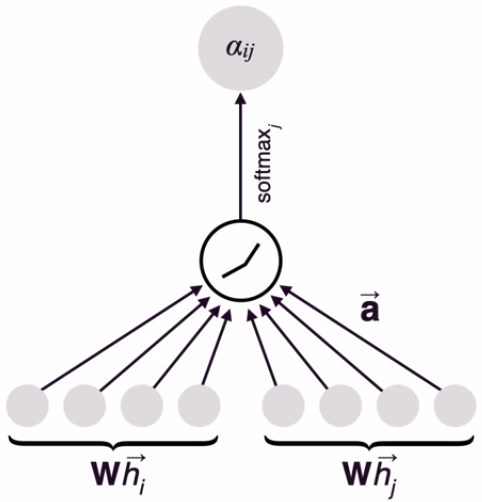
\includegraphics[width=0.65\textwidth]{figures/GAT_step_1.png}
                \caption{Attention mechanism. It looks at features of node $i$ and its neighbor $j$, then the attention function computes the coefficient $\alpha_{ij}$, which signifies the influence of node $i$ to node $j$.}
                \label{fig:GAT_step_1}
            \end{figure}
        \end{column}
        
        \begin{column}{.5\textwidth}
            \begin{figure}
                \centering
                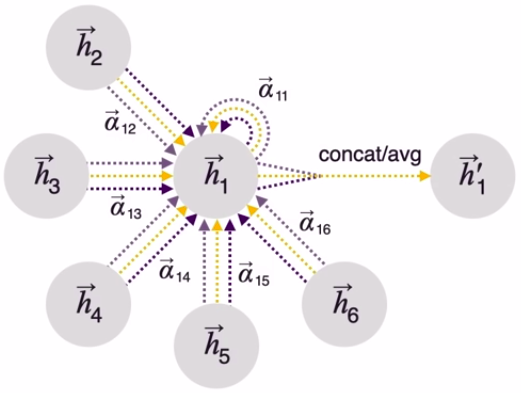
\includegraphics[width=0.8\textwidth]{figures/GAT_step_2.png}
                \caption{Multi-head attention mechanism. Each colored line indicates a different way in which the node receives information from its immediate neighbors, which is aggregated to produce an updated representation.}
                \label{fig:GAT_step_2}
            \end{figure}
        \end{column}
    \end{columns}
    \footnotesize{Images from \cite{PetarIntroGNN}}
\end{frame}


\begin{frame}{Graph Pooling}

    What if we want to learn an embedding $\mathbf z_G$ for the entire graph $G$? $\longrightarrow$ \alert{graph pooling}
    
    We want to design a pooling function $f_p$, which maps a set of node embeddings $\{\mathbf z_1, \ldots, \mathbf z_{|V|} \}$ to an embedding $\mathbf z_G$ that represents the full graph.
    
    One approach is to simply to take a sum (or mean) of the node embeddings:
    \begin{equation}
        \mathbf z_G = \frac{\sum_{v \in V} \mathbf z_u}{f_n(|V|)},
    \end{equation}
    where $f_n$ is some normalizing function (e.g., the identity function, so $\mathbf z_G = (\sum_{v \in V} \mathbf z_u)/|V|$).
    \bigskip
    
    \textbf{Limitation}: it does not exploit the structure of the graph! We want to exploit the graph topology at the pooling stage. $\longrightarrow$ use \alert{graph clustering or coarsening}
    
\end{frame}


\begin{frame}{Generalized Message Passing}

    The presentation in this chapter so far has focused on the most popular style of GNN message passing, which operates largely at the node level. However, the GNN message passing approach can also be generalized to leverage edge and graph-level information at each stage of message passing. For example, in the more general approach proposed by \cite{battaglia2018relational}, we define each iteration of message passing according to the following equations:
    \begin{align}
        \mathbf h^{(k)}_{(u,v)} &= \textsc{update}_\text{edge} (\mathbf h_{(u,v)}^{(k-1)}, \mathbf h_u^{(k-1)}, \mathbf h_v^{(k-1)}, \mathbf h_G^{(k-1)})
        \label{eq:upedge} \\
        \mathbf m_{\mathcal N(u)} &= \textsc{aggregate}_\text{node}(\{ \mathbf h_{(u,v)}^{(k)}, \; \forall v \in \mathcal N(u) \})
        \label{eq:message} \\
        \mathbf h^{(k)}_u &= \textsc{update}_\text{node} ( \mathbf h_u^{(k-1)}, \mathbf m_{\mathcal N(u)}, \mathbf h_G^{(k-1)})
        \label{eq:upnode} \\
        \mathbf h^{(k)}_G &= \textsc{update}_\text{graph}(\mathbf h_G^{( k-1)}, \{ \mathbf h_u^{(k)}, \, \forall u \in V\}, \{ \mathbf h_{(u,v)}^{(k)}, \forall (u, v) \in E\}).
        \label{eq:upgraph}
    \end{align}
    The important innovation in this generalized message passing framework is that, during message passing, we generate hidden embeddings $\mathbf h_{(u,v)}^{(k)}$ for each edge in the graph, as well as an embedding $h_G^{(k)}$ corresponding to the entire graph. This allows the message passing model to easily integrate edge and graph-level features, and recent work has also shown this generalized message passing approach to have benefits compared to a standard GNN in terms of logical expressiveness. Generating embeddings for edges and the entire graph during message passing also makes it trivial to define loss functions based on graph or edge-level classification tasks.
    
\end{frame}


\begin{frame}[allowframebreaks]{Graph Neural Networks in Practice}

    In the vast majority of current applications, GNNs are used for one of three tasks: node classification, graph classification, or relation prediction.
    \begin{itemize}
        \item[\alert{$\bullet$}] \emph{GNNs for Node Classification} $\rightarrow$ train GNNs in a fully-supervised manner with a negative log-likelihood loss:
        \begin{equation}
            \mathcal L = \sum_{u \in V_\text{train}} -\log(\text{softmax}(\mathbf z_u, \mathbf y_u)),
        \end{equation}
        where $\mathbf y_u$ is a one-hot vector indicating the class of training node $u \in V_\text{train}$ and $\text{softmax}(\mathbf z_u, \mathbf y_u)$ denotes the predicted probability that the node belongs to the class $\mathbf y_u$, computed via the $\text{softmax}$ function:
        \begin{equation}
            \text{softmax}(\mathbf z_u, \mathbf y_u) = \sum^c_{i=1} \mathbf y_u[i] \frac{e^{\mathbf z_u^\top \mathbf w_i}}{\sum^c_{j=1} e^{\mathbf z_u^\top \mathbf w_j}},
            \label{eq:lossnodeclass}
        \end{equation}
        where $\mathbf w_i \in \mathbb R^d, i = 1, \ldots, c$ are trainable parameters.
        
        \item[\alert{$\bullet$}] \emph{GNNs for Graph Classification} $\rightarrow$ a softmax classification loss --- analogous to \autoref{eq:lossnodeclass} --- is often used, with the key difference that the loss is computed with graph-level embeddings $\mathbf z_{G_i}$ over a set of labeled training graphs $\mathcal G = \{G_1, \ldots, G_n\}$. In recent years, GNNs have also witnessed success in regression tasks involving graph data. In these instances, it is standard to employ a squared-error loss of the following form:
        \begin{equation}
            \mathcal L = \sum_{G_i \in \mathcal G} \| \textbf{MLP}(\mathbf z_{G_i}) - y_{G_i}\|_2^2,
        \end{equation}
        where $\textbf{MLP}$ is a densely connected neural network with a univariate output and $y_{G_i} \in \mathbb R$ is the target value for training graph $G_i$.
        
        \item[\alert{$\bullet$}] \emph{GNNs for Edge Prediction} $\rightarrow$ While classification tasks are by far the most popular application of GNNs, GNNs are also used in in edge prediction tasks, such as recommender systems and knowledge graph completion. In these applications, the standard practice is to employ the pairwise node embedding loss functions. In principle, GNNs can be combined with any of the pairwise loss functions discussed previously, with the output of the GNNs replacing the shallow embeddings.
    \end{itemize}
\end{frame}


\begin{frame}{Relational inductive biases in graph networks}

    Our GN framework imposes several strong relational inductive biases when used as components in a learning process.
    First, graphs can express arbitrary relationships among entities, which means the GN's input determines how representations interact and are isolated, rather than those choices being determined by the fixed architecture. For example, the assumption that two entities have a relationship---and thus should interact---is expressed by an edge between the entities' corresponding nodes. Similarly, the absence of an edge expresses the assumption that the nodes have no relationship and should not influence each other directly. 
    
    Second, graphs represent entities and their relations as sets, which are invariant to permutations. This means GNs are invariant to the order of these elements\footnote{Note, an ordering can be imposed by encoding the indices in the node or edge attributes, or via the edges themselves (e.g. by encoding a chain or partial ordering).}, which is often desirable.
    For example, the objects in a scene do not have a natural ordering (see Sec.~\ref{sec:sets-and-graphs}).
    
    Third, a GN's per-edge and per-node functions are reused across all edges and nodes, respectively. This means GNs automatically support a form of combinatorial generalization (see Section~\ref{sec:combinatorial-generalization}): because graphs are composed of edges, nodes, and global features, a single GN can operate on graphs of different sizes (numbers of edges and nodes) and shapes (edge connectivity).
    
\end{frame}


{\putbg
\section{Combinatorial Optimization and Reasoning with GNN}}


{\putbgdark
\begin{frame}[standout]
	\begin{center}
		\Large \uncover<+->{Thank you for your attention!}
		
		\Huge\uncover<+->{\Smiley}
	\end{center}
\end{frame}
}

\begin{frame}[allowframebreaks]{}

	\nocite{*}
	\printbibliography

\end{frame}

\end{document}